\chapter{Querying and Validating Information for GDPR Compliance}
\label{chapter:testing}
% chapter introduction
This chapter presents the application of semantic web technologies to query and validate information for GDPR compliance.
It represents information using the developed vocabularies of GDPRtEXT, GDPRov, and GConsent presented in \autoref{chapter:vocabularies}.
The queries are represented using SPARQL - a W3C standard for querying RDF - and are based on the compliance questions presented in \autoref{sec:info:compliance-questions}.
Validation is carried out based on the identified assumptions and constraints presented in \autoref{sec:info:constraints} and is expressed using SHACL which is the W3C standard for representing constraints.
The presented work represents minor contributions of this thesis, and fulfils the research objective $RO4$ regarding querying of information and $RO5$ regarding validation of information for GDPR compliance.

\section{Querying Information for GDPR Compliance using SPARQL}\label{sec:testing:sparql}
This section presents the creation and utilisation of SPARQL queries to retrieve information relevant for GDPR compliance.
The creation of the queries is dependant on the ontological representation of information being retrieved, which in this case includes the use of GDPRov and GDPRtEXT ontologies. This is further explained in \autoref{sec:testing:sparql:relation}
A GDPR preparation guide published by the Irish Data Protection Commission was used as the source of compliance questions for which corresponding the SPARQL queries were created. The methodology used for this is presented in \autoref{sec:testing:sparql:methodology} with an demonstration of the developed queries presented in \autoref{sec:testing:sparql:demo}.
A note on the evaluation of this work is presented in \autoref{sec:testing:sparql:evaluation}.

\subsection{SPARQL queries and ontological representation of information}\label{sec:testing:sparql:relation}
The research regarding querying presented here is based on the task of retrieving information for answering questions relevant to the assessment of compliance.
It represents utilisation of technical solutions to automate the task of information retrieval and requires machine-readable data (or metadata).
For this, the developed vocabularies provide the ontological concepts and relationships necessary to express the information using GDPR terminology and enable the association of information with clauses and concepts of GDPR.

The compliance questions, as presented in \autoref{sec:info:compliance-questions}, do not use a specific ontology or vocabulary but instead are based in the natural language and use legal terminology. In order to utilise technological solutions for answering them, it is necessary to first convert these questions into queries which can be executed over the compliance representation.
Since the work presented in this thesis derives motivation from the use of semantic web technologies which use RDF for representing information, the task of querying utilises the SPARQL standard to retrieve this information.

The ontology used in the SPARQL queries must match the ontology used in the representation of information associated with compliance. Differences in ontologies would hamper the effective of execution of queries and have the potential to return invalid results or empty results.
The creation of SPARQL queries is therefore specific to the ontologies used in a particular information representation, and is therefore also specific to the use-case it is used in.

\subsection{Methodology}\label{sec:testing:sparql:methodology}
The methodology used for creation of SPARQL queries is based on utilisation of GDPRov to represent the concepts and GDPRtEXT to link the information to the GDPR.
The SPARQL queries thus created aim to retrieve information relevant to answering the question rather than present an evaluation or assessment of compliance.
While the compliance questions presented in \autoref{sec:info:compliance-questions} provide a basis for construction of semantic queries using SPARQL, we focused on identifying a real-world use-case of the use of such compliance questions to provide a demonstration of the application of this research.

\subsubsection{Utilising compliance questions from GDPR readiness guide published by DPC}
We utilised the guide titled ``Preparing Your Organisation for the GDPR – A Guide for SMEs'' published by Data Protection Commission of Ireland (DPC) as the basis for compliance questions which were represented using SPARQL as semantic queries.
The guide was published by the DPC in 2017 to help organisations in assessing their readiness towards GDPR compliance requirements.
It is accessible online\footnote{\url{http://gdprandyou.ie/wp-content/uploads/2017/12/A-Guide-to-help-SMEs-Prepare-for-the-GDPR.pdf}} and consists of a `table' (see Fig. \ref{fig:sparql:guide}) containing questions regarding information about an organisations processing activities.
The guide divides the questions into contextual sections based on addressing specific GDPR articles and obligations.
\begin{figure}[htbp]
\centering
\fbox{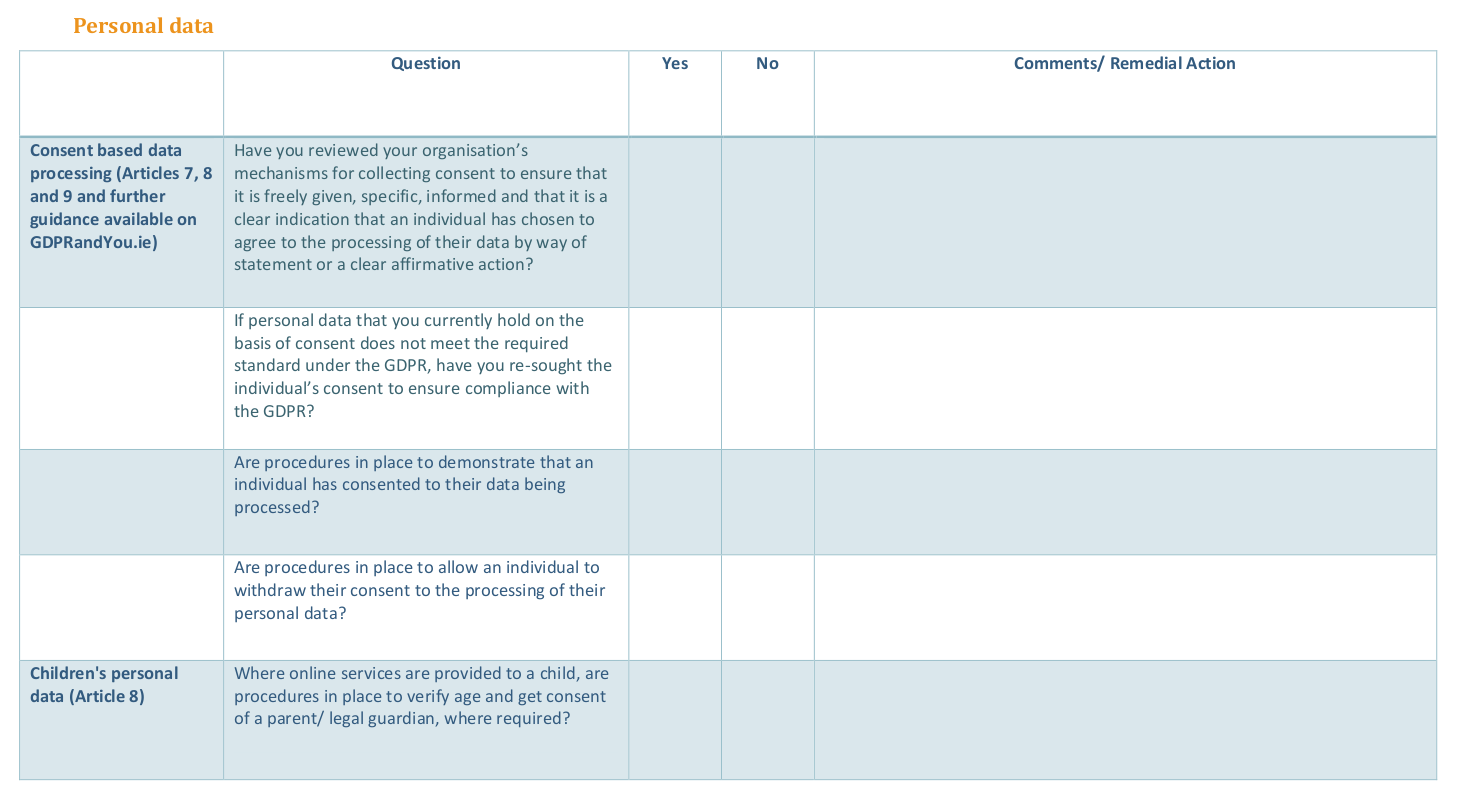
\includegraphics[width=\textwidth]{img/GDPR_guide_page_10.png}}
\caption{Questions for information required to assess compliance - Page 10 of ``Preparing Your Organisation for the GDPR - A Guide for SMEs'' published by Ireland's Data Protection Commission}
\label{fig:sparql:guide}
\end{figure}

\subsubsection{Steps of the methodology}
The steps followed in utilising the questions in the guide to create SPARQL queries and demonstrate their application were as follows:
\begin{enumerate}
    \item Analyse questions within the document to identify corresponding concepts and relationships in GDPRov and GDPRtEXT (see below)
    \item Represent questions as SPARQL queries using GDPRov and GDPRtEXT (see below)
    \item Create a synthetic use-case based on processing of personal data with GDPRov and GDPRtEXT used to represent information (see \autoref{sec:testing:sparql:demo})
    \item Execute SPARQL queries over use-case to retrieve answers for compliance questions (see \autoref{sec:testing:sparql:demo})
    \item Evaluate the queries based on the subjective criteria of - a) Extent of answering compliance questions b) Suitability of retrieved results in answering compliance questions (see \autoref{sec:testing:sparql:evaluation})
\end{enumerate}

\subsubsection{Analysis of GDPR Readiness Guide}
The guide contains 63 questions across 13 pages that are presented in 9 sections.
Its analysis consisted of categorising the questions based on requirements of information, relation to phases of compliance, and whether they were suitable to be implemented as SPARQL queries.
The analysis was recorded and published online\footnote{\url{https://w3id.org/GDPRep/checklist-demo/notes}} in the form of a spreadsheet with comments describing the thought process in interpreting each question's information requirements.

The first set of questions on page 1 concern consent and personal data and are structurally different than the other set of questions in that they are more abstract and generic and concern the overall practices concerning processing of personal data by the organisation.
These questions are described under the `general' category with other groups of questions having their category mentioned explicitly within the document.
Questions in the general category require information and practices associated with consent and personal data. Other categories contain questions which enquire explicitly about activities and mechanisms regarding compliance to specific obligations.

The questions were analysed and categorised into three categories based on their intended requirements towards information required for compliance. The three categories identified through this exercise were - demonstrative, evaluative, and assistive - based on the requirements of information associated with them. 
Demonstrative questions require answers that satisfy the compliance question and do not need further actions or processing based on the information. 
Assistive questions provide information that can be directly evaluated for compliance, with the term `assistive' indicating information that assists in the evaluation.
Evaluative questions retrieve information whose evaluation requires further information retrieved through additional questions based on the provided information.
The primary difference assistive and evaluative questions is whether they retrieve information which can be evaluated as is for compliance or whether it requires additional questions to retrieve further information.
These terms used for categorisation are arbitrary and do not relate to any specific methodology for legal compliance, but are useful to analyse the question from an information management perspective.

Questions were also analysed based on whether they relate to or require information regarding activities in ex-ante and ex-post phases.
The questions do not explicitly provide an indication of whether they enquire about a model of processing (ex-ante) or the execution (ex-post). The distinction was based on whether the question concerned information about practices, plans, or intentions regarding processing of personal data - in which case it was deemed to enquire about ex-ante information.
Similarly, if a question concerned past execution of activities or records of activities - it was said to enquire about ex-post information.
In some cases, questions were specified to enquire about both ex-ante and ex-post information based on potential application in both phases.

An overview of the questions is provided in \autoref{table:sparql:dpc-1}.
It assigns an ID for each question to enable associating it with the corresponding SPARQL query and for linking related questions in the analysis.
The column `\textit{Category}' reflects the category of question mentioned within the guide, with general used for the initial generic questions.
`\textit{Title}' refers to the title of the text within the guide, and the column `\textit{GDPR}' refers to an explicit mention of a GDPR clause within the question or its description.
\begin{table}[htbp]
\footnotesize
\centering
\caption{Questions provided in the GDPR Readiness Guide}
\begin{tabularx}{\textwidth}{|l|l|X|l|}
\hline
ID & Category & Title & GDPR \\ \hline
G1 & General & Categories of personal data and data subjects &  \\ \hline
G2 & General & Elements of personal data included within each data category &  \\ \hline
G3 & General & Source of the personal data &  \\ \hline
G4 & General & Purposes for which personal data is processed &  \\ \hline
G5 & General & Legal basis for each processing purpose (non-special categories of personal data) &  \\ \hline
G6 & General & Special categories of personal data &  \\ \hline
G7 & General & Legal basis for processing special categories of personal data &  \\ \hline
G8 & General & Retention period &  \\ \hline
G9 & General & Action required to be GDPR compliant? &  \\ \hline
P1 & PersonalData & Validity of Consent & 7,8,9 \\ \hline
P2 & PersonalData & Retrospective Consent & 7,8,9 \\ \hline
P3 & PersonalData & Demonstration of Consent & 7,8,9 \\ \hline
P4 & PersonalData & Withdraw consent for processing & 7.8.9 \\ \hline
P5 & PersonalData & Children's Personal Data & 8 \\ \hline
P6 & PersonalData & Legitimate interest based data processing &  \\ \hline
R1 & Rights & Subject Access Requests (SARs) & 15 \\ \hline
R2 & Rights & Subject Access Requests (SARs) Response Time & 15 \\ \hline
R3 & Rights & Data Portability & 20 \\ \hline
R4 & Rights & Deletion and Rectification & 16,17 \\ \hline
R5 & Rights & Right to restriction of processing & 18 \\ \hline
R6 & Rights & Right to object to processing & 21 \\ \hline
R7 & Rights & Halt processing after right to object & 21 \\ \hline
R8 & Rights & Profiling and automated processing & 22 \\ \hline
R9 & Rights & Right to obtain human intervention & 22 \\ \hline
R10 & Rights & Restrictions to data subject rights & 23 \\ \hline
A1 & AccuracyRetention & Purpose Limitation &  \\ \hline
A2 & AccuracyRetention & Data minimisation &  \\ \hline
A3 & AccuracyRetention & Accuracy &  \\ \hline
A4 & AccuracyRetention & Retention &  \\ \hline
A5 & AccuracyRetention & Retention Legal Obligations &  \\ \hline
A6 & AccuracyRetention & Destroy data securely &  \\ \hline
A7 & AccuracyRetention & Duplication of records &  \\ \hline
T1 & Transparency & Transparency to customers and employees & 12,13,14 \\ \hline
T2 & Transparency & Provide Information listed in Article 13 & 13 \\ \hline
T3 & Transparency & Provide Information listed in Article 14 & 14 \\ \hline
T4 & Transparency & Provide information when engaging &  \\ \hline
T5 & Transparency & Provide information on facilitating rights &  \\ \hline
C1 & ControllerObligations & Supplier Agreements & 27,28,29 \\ \hline
C2 & ControllerObligations & Data Protection Officers & 37,38,39 \\ \hline
C3 & ControllerObligations & Reasons for not having a DPO & 37,38,39 \\ \hline
C4 & ControllerObligations & Escalation procedures & 37,38,39 \\ \hline
C5 & ControllerObligations &  & 37,38,39 \\ \hline
C6 & ControllerObligations & Data Protection Impact Assessments (DPIAs) & 35 \\ \hline
S1 & DataSecurity & Risks involved in processing data & 32 \\ \hline
S2 & DataSecurity & Documented Security Program & 32 \\ \hline
S3 & DataSecurity & Resolving security related issues & 32 \\ \hline
S4 & DataSecurity & Designated individual for security & 32 \\ \hline
S5 & DataSecurity & Encryption & 32 \\ \hline
S6 & DataSecurity & Removing information & 32 \\ \hline
S7 & DataSecurity & Restoring access & 32 \\ \hline
B1 & DataBreach & Documented incident plans & 33,34 \\ \hline
B2 & DataBreach & Regular reviews & 33,34 \\ \hline
B3 & DataBreach & Notifying authorities & 33,34 \\ \hline
B4 & DataBreach & Notifying data subjects & 33,34 \\ \hline
B5 & DataBreach & Documentation of data breaches & 33,34 \\ \hline
B6 & DataBreach & Co-operation procedures for data breach & 33,34 \\ \hline
I1 & InternationalDataTransfer & Data transfer outside EEA & 44,45,46,47,48,49,50 \\ \hline
I2 & InternationalDataTransfer & Special category of Personal Data in Transfer & 44,45,46,47,48,49,50 \\ \hline
I3 & InternationalDataTransfer & Purpose of Transfer & 44,45,46,47,48,49,50 \\ \hline
I4 & InternationalDataTransfer & Transfer Recipients & 44,45,46,47,48,49,50 \\ \hline
I5 & InternationalDataTransfer & Transfer Details & 44,45,46,47,48,49,50 \\ \hline
I6 & InternationalDataTransfer & Legality of international transfers &  \\ \hline
I7 & InternationalDataTransfer & Transparency &  \\ \hline

\end{tabularx}
\label{table:sparql:dpc-1}
\end{table}

\autoref{table:sparql:dpc-2} presents a summarised view of the analysis of compliance questions presented in \autoref{table:sparql:dpc-1}.
The complete information along with additional comments and fields is available in the online published version of the analysis.
In the table, column `\textit{Type}' indicate the type of query based on categorisation as demonstrative, assistive, evaluative based on the description in the sections above.
The column `\textit{Data}' provides information on information required for the question, including results of other queries.
The relation of question to the ex-ante phase of compliance is reflected by the column `\textit{E/A}' and ex-post phase by the column '\textit{E/P}' using boolean \texttt{Y/N} values.
The column `\textit{SPARQL}' indicates whether a SPARQL query was constructed for the corresponding question.
The column `\textit{GDPRov}' indicates whether the current iteration of GDPRov provides the necessary concepts and relationships to answer the compliance question, with a value of \texttt{Y} indicating that it does, \texttt{N} indicating it does not, and \texttt{S} indicating the information to be out of scope for GDPRov.
\begin{table}[htbp]
\footnotesize
\centering
\caption{Analysis of compliance questions specified in \autoref{table:sparql:dpc-1}}
\begin{tabularx}{\textwidth}{|l|l|X|l|l|l|l|}
\hline
ID & Type & Data & E/A & E/P & SPARQL & GDPRov \\ \hline
G1 & Demn & personal data, data subjects & Y & N & Y & Y \\ \hline
G2 & Demn & personal data & Y & N & Y & Y \\ \hline
G3 & Demn & personal data, steps that collect data, entities that provde data & Y & Y & Y & Y \\ \hline
G4 & Demn & results of G1, processes acting on data & Y & N & Y & Y \\ \hline
G5 & Demn & results of G4, processes acting on data & Y & N & Y & Y \\ \hline
G6 & Demn & special category personal data & Y & N & Y & Y \\ \hline
G7 & Demn & results of G6, steps that collect data, steps that store data & Y & N & Y & Y \\ \hline
G8 & N/I & results of G1, steps that store data &  &  & N & E \\ \hline
G9 & N/I &  &  &  & N & N \\ \hline
P1 & Asst & consent, steps that acquire consent & Y & N & Y & S \\ \hline
P2 & N/I &  &  &  & N & S \\ \hline
P3 & Eval & consent & Y & Y & Y & Y \\ \hline
P4 & Eval & steps that withdraw consent & Y & N & Y & Y \\ \hline
P5 & Eval & steps that acquire consent, steps for age verification & Y & N & Y & Y \\ \hline
P6 & Asst & steps that process personal data & Y & N & Y & Y \\ \hline
R1 & Asst & steps that handle SAR & Y & N & Y & Y \\ \hline
R2 & Asst & steps that handle SAR & N & Y & N & Y \\ \hline
R3 & Eval & steps that address right to data portability & Y & N & Y & Y \\ \hline
R4 & Eval & steps that address right to rectification & Y & N & Y & Y \\ \hline
R5 & Asst & data subjet request, steps that process personal data & N & Y & N & Y \\ \hline
R6 & N/I &  &  &  & N & Y \\ \hline
R7 & Eval & steps that process personal data & Y & N & Y & Y \\ \hline
R8 & Asst & steps that make automated decisions, consent & Y & Y & Y & Y \\ \hline
R9 & Asst & steps that make automated decisions, right to contest automated decisions & Y & N & Y & Y \\ \hline
R10 & N/I &  &  &  & N & S \\ \hline
A1 & Eval & personal data, consent, steps that involve personal data through use, share, store & Y & Y & Y & S \\ \hline
A2 & Asst & personal data, steps that process personal data & Y & Y & Y & S \\ \hline
A3 & N/I &  &  &  & N & S \\ \hline
A4 & N/I &  &  &  & N & S \\ \hline
A5 & N/I &  &  &  & N & S \\ \hline
A6 & Asst & steps that delete data & Y & N & Y & N \\ \hline
A7 & N/I &  &  &  & N & S \\ \hline
T1 & N/I &  &  &  & N & S \\ \hline
T2 & Asst & steps that collect personal data & Y & N & Y & N \\ \hline
T3 & Asst & steps that collect personal data & Y & N & Y & N \\ \hline
T4 & N/I &  &  &  & N & S \\ \hline
T5 & N/I &  &  &  & N & N \\ \hline
C1 & N/I &  &  &  & N & N \\ \hline
C2 & N/I &  &  &  & N & Y \\ \hline
C3 & N/I &  &  &  & N & S \\ \hline
C4 & N/I &  &  &  & N & N \\ \hline
C5 & N/I &  &  &  & N & N \\ \hline
C6 & Asst & steps part of the DPIA process & Y & N & Y & N \\ \hline
S1 & Asst & steps that process data & Y & N & Y & S \\ \hline
S2 & N/I &  &  &  & N & N \\ \hline
S3 & N/I &  &  &  & N & N \\ \hline
S4 & N/I &  &  &  & N & N \\ \hline
S5 & N/I & steps that share data &  &  & N & N \\ \hline
S6 & N/I &  &  &  & N & N \\ \hline
S7 & N/I &  &  &  & N & N \\ \hline
B1 & Eval & processes or plan that address security incidents & Y & N & Y & N \\ \hline
B2 & N/I &  &  &  & N & N \\ \hline
B3 & Eval & processes or plans for notifying DPC & Y &  & Y & Y \\ \hline
B4 & Eval & processes or plans for notifying data subjects of a data breach &  &  & Y & Y \\ \hline
B5 & N/I &  &  &  & N & Y \\ \hline
B6 & N/I &  &  &  & N & N \\ \hline
I1 & Eval & steps that share data & Y & Y & Y & Y \\ \hline
I2 & Eval & results from I1, category of personal data & Y & N & Y & Y \\ \hline
I3 & Asst & steps that share data & Y & Y & Y & Y \\ \hline
I4 & Eval & steps that share data & Y & Y & Y & Y \\ \hline
I5 & N/I &  &  &  & N & Y \\ \hline
I6 & N/I &  &  &  & N & Y \\ \hline
I7 & N/I & steps that share data &  &  & N & S \\ \hline
\end{tabularx}
\label{table:sparql:dpc-2}
\end{table}

% Where the questions could not be answered due to missing concepts and relationships in GDPRov, or due to uncertain interpretations of a legal concept or ambiguity, a note was made to identify solutions in the future.
% This was used to update the GDPRov at a later date with additional concepts, such as for legal bases, data sharing, data transfers, or documentation of data breaches.
The information regarding GDPRov is also provided since the creation of SPARQL queries from GDPR readiness guide was carried out in the earlier stages of GDPRov's iterations and before the enforcement of the GDPR in May 2018. Therefore, some questions were deemed to be ambiguous or lacking legal information on information necessary for compliance.
The queries and constraints presented in \autoref{sec:testing:shacl} were developed at a later stage when GDPR had seen significant attention and interpretation and do not suffer from similar absences of implementation.
Since the aim of the exercise was in demonstrating usefulness of SPARQL to represent compliance questions, and the minor role of such queries in the contributions of this research, this gap was rectified in future applications rather than the current one.

\subsubsection{Creation of SPARQL queries}
The creation of SPARQL queries involved analysis of the text of a question to identify relevant concepts and relationships in GDPRov useful towards expressing the question as a semantic query in SPARQL as well as representing the information required to answer the question.
In this, some questions were found to be subjective or qualitative and thus could not be expressed as SPARQL queries. These are indicated as not implemented in \autoref{table:sparql:dpc-2} and were also included in the webpage of implementation presented in \autoref{sec:testing:sparql:demo}.

A total of 33 SPARQL queries were created based on the above analysis of compliance questions and their requirements.
The queries utilised GDPRov and GDPRtEXT ontologies to specify the information associated with the question.
The SPARQL queries were published online\footnote{\url{https://w3id.org/GDPRep/checklist-demo/sparql-queries}}
with a seperate files for each query associated with a compliance question, and a common file containing the common prefixes used in all queries.

As an example, Listing \autoref{code:sparql:dpc-G5} contains the corresponding SPARQL query for compliance question \texttt{G5} which concerns the legal basis used to justify processing of personal data. 
The query retrieves information about steps and the processes along with the legal basis for their operation in ex-ante phase using the vocabulary provided by GDPRov.
Within this, the query specifically retrieves steps which are defined as being part of a process and use some form of personal data. 
The legal bases can be associated with individual steps or with the process they are associated with.
\begin{listing}[ht]
\begin{minted}[
    frame=single,
    framesep=5mm,
    baselinestretch=1,
    linenos
]{text}
PREFIX rdfs:     <http://www.w3.org/2000/01/rdf-schema#>
PREFIX gdprov:   <http://purl.org/adaptcentre/openscience/ontologies/gdprov#>
PREFIX gdprtext: <http://purl.org/adaptcentre/openscience/ontologies/GDPRtEXT#>

SELECT DISTINCT ?process ?legal WHERE {
  ?data a ?data_type .
  ?data_type rdfs:subClassOf gdprov:PersonalData .
  ?step a ?step_type .
  ?step_type rdfs:subClassOf gdprov:DataStep .
  ?step gdprov:usesData ?data . 
  ?step gdprov:isPartOfProcess ?process .
  OPTIONAL { ?step gdprov:hasLegalBasis ?legal } .
  OPTIONAL { ?process gdprov:hasLegalBasis ?legal } .
} ORDER BY ?process
\end{minted}
\caption{SPARQL query representing compliance question \texttt{G5} concerning legal basis for processing}
\label{code:sparql:dpc-G5}
\end{listing}

\subsection{Demonstration using synthetic use-case}\label{sec:testing:sparql:demo}


\subsection{Evaluation}\label{sec:testing:sparql:evaluation}

\subsection*{Conclusion}

\section{Validating Information for GDPR Compliance using SHACL}\label{sec:testing:shacl}

\subsection{Methodology}\label{sec:testing:shacl:methodology}

\subsection{Creation of SHACL constraints}\label{sec:testing:shacl:constraints}

\subsection{Exploring combination of ex-ante and ex-post validations}\label{sec:testing:shacl:combine}

\subsubsection{Exploring creation of a compliance graph}\label{sec:testing:shacl:compliance-graph}

\subsection{Demonstrating using use-case of consent given on a website}\label{sec:testing:shacl:demo}

\subsection{Evaluation}\label{sec:testing:shacl:eval}

\subsection*{Conclusion}

\section*{Chapter Summary}